\documentclass[]{report}

\usepackage[utf8]{inputenc}
\usepackage[spanish]{babel}
\usepackage{graphicx}
\graphicspath{{imagenes/}}
\usepackage[colorlinks]{hyperref}
\usepackage[svgnames]{xcolor}
\hypersetup{citecolor=DarkRed}
\hypersetup{linkcolor=DarkBlue}
\hypersetup{urlcolor=DarkBlue}

% Title Page
\title{Agrupamiento difuso}
\author{Carlos Cobos Suárez\\Adrián Morente Gabaldón}


\begin{document}
\maketitle

\begin{abstract}
	
	Este trabajo versa sobre el ámbito de la ciencia de datos y consiste en exponer las limitaciones del agrupamiento o \textit{clustering} clásico para resolverlas tras estudiar cómo la lógica difusa puede ayudar en la modelización del problema.\\
	
	Se darán a conocer los distintos tipos de modelos de agrupamiento usando lógica difusa, así como sus características y limitaciones intentando resolverlas con otro tipo de modelos.\\
	
	Para terminar y entender que los modelos expuestos tienen una gran relevancia en nuestra sociedad, así cómo destacar cómo el agrupamiento difuso (o \textit{fuzzy clustering}) está presente en nuestros días, se citarán aplicaciones reales que hacen uso de estos modelos.\\
	
\end{abstract}

	\chapter{Agrupamiento clásico}
	
		\section{Definición}
		
			Entendemos por \textbf{agrupamiento clásico} a la técnica de clasificación de datos en distintas categorías según su similitud (o \textit{distancia}, si los entendemos como una representación de puntos en un espacio determinado).
			
			\begin{figure}[h]
				\centering
				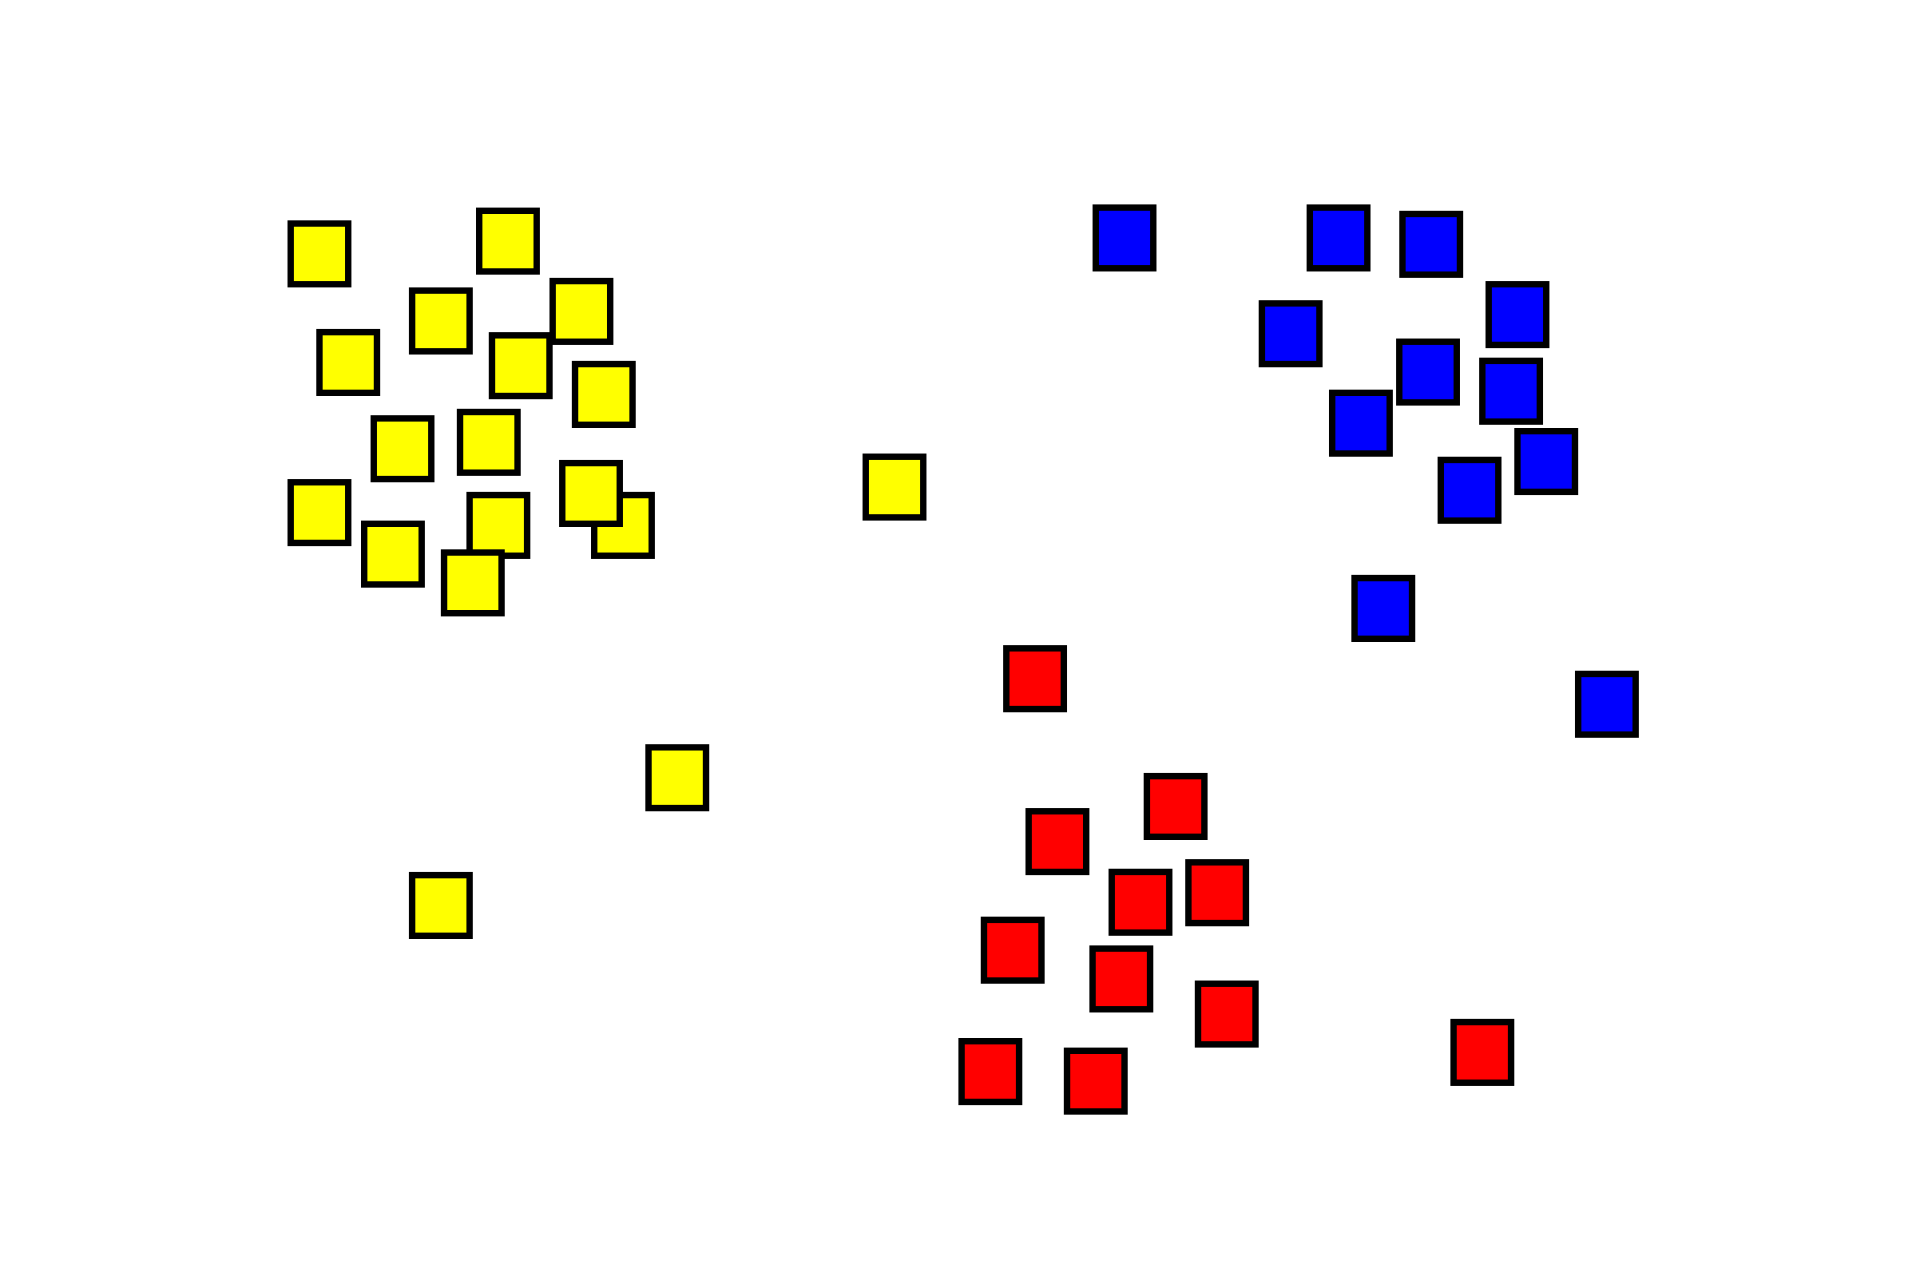
\includegraphics[width=0.5\textwidth]{clustering.png}
				\label{clustering1}
				\caption{Ilustración de agrupamiento clásico. \href{https://en.wikipedia.org/wiki/Cluster_analysis\#/media/File:Cluster-2.svg}{ \textit{(Wikimedia Creative Commons)}}}
			\end{figure}
		
			Se trata de una tarea principal en la labor de minería de datos a modo exploratorio, además de una técnica común para análisis estadístico de datos (aprendizaje automático, reconocimiento de patrones, análisis de imágenes, etc.).
					
		\section{Conceptos}
		
			Para entender con mayor profundidad los fundamentos del \textit{clustering}, deben interiorizarse algunos conceptos clave:
			
			\begin{itemize}
				\item \textbf{Clúster \textit{(o cluster)}}: se trata de cada una de las categorías o grupos en los que se clasifican finalmente los datos. Esto es, según vemos en la figura \ref{clustering1}, los distintos colores que identifican a cada grupo.
				\item \textbf{Centroide}: se conoce como tal al punto de referencia de cada \textit{cluster}, es decir, el elemento más representativo que comparte mayor similitud con el resto.
				\item \textbf{Función de distancia}: es la relación que indica el grado de disimilaridad entre los elementos del conjunto analizado; siendo mayor la similitud entre ellos cuanto menor sea esta \textit{distancia}, considerando a los individuos como vectores en el espacio de las variables. Puede calcularse mediante \textit{distancia euclídea}, \textit{distancia Hamming} o \textit{correlación de Pearson} entre otras.
				\item \textbf{Núcleo o \textit{kernel}}: son clases de algoritmos para análisis de patrones, donde la tarea general es encontrar y estudiar tipos de relaciones en conjuntos de datos. En su definición más simple, implican la transformación de datos en otras dimensiones cuyo margen divisorio de los elementos es más acentuado y permite una visualización y categorización más claras.
			\end{itemize}
		
		\section{Modelos de agrupamiento clásico}
		
			Durante el estudio de conjuntos de datos basado en agrupamientos y/o categorización, se pueden seguir diversos modelos que condicionarán el contenido de los grupos resultantes. Esto es, el resultado diferirá en función del criterio seguido para asignar una categoría u otra a cada uno de los datos presentes en el conjunto. Veamos algunos de los modelos posibles:
		
			\begin{itemize}
				\item \textbf{Conectividad}: el criterio seguido para categorizar cada uno de los elementos se corresponde con la cercanía que tenga un determinado dato con el resto. Por ejemplo, si en un espacio tridimensional un dato sin categoría se encontrase a una distancia euclídea de 10 de un elemento de clase A, y a una distancia 5 de un dato de clase B; se inferiría que el elemento estudiado comparte más similitud con los datos de la segunda clase, y se categorizaría dentro de ella.
				\item \textbf{Basado en centroide}: en este caso, se seguiría una especie de modelo guiado por conectividad con la salvedad de que las distancias se calcularían respecto a cada uno de los centroides presentes en el modelo, y dicho elemento se clasificaría dentro de la clase a la que está asignado el centroide más cercano.
				\item \textbf{Basado en distribuciones}: es el más estrechamente ligado a los modelos y fundamentos estadísticos. Los clústeres son definidos por objetos que pertenecen mayormente a la misma distribución. Producen modelos complejos con que capturar correlación y dependencia entre atributos de los datos estudiados. A menos que se establezcan unos límites sobre la complejidad del modelo, el \textit{sampling} de datos aleatorios de forma estadística puede afectar negativamente causando \textbf{sobreajuste}.
				\item \textbf{Basado en densidad}: en este modelo, los grupos son definidos a modo de áreas donde la densidad de datos es mayor que en el resto del conjunto. Los objetos que se encuentran esparcidos por el espacio sin acercarse a ningún área, se consideran \textit{ruido} o \textbf{puntos frontera}.
			\end{itemize}
		
		\section{Proceso y algoritmo}
		
			El proceso de clasificación de datos en clases es relativamente sencillo, y se puede explicar de forma ejemplificada según el conocido algoritmo \textbf{\textit{K-means}} (o \textit{K-medias} en español), que asigna clases a los datos no categorizados en función del centroide más cercano:
		
			\begin{figure}[h]
				\centering
				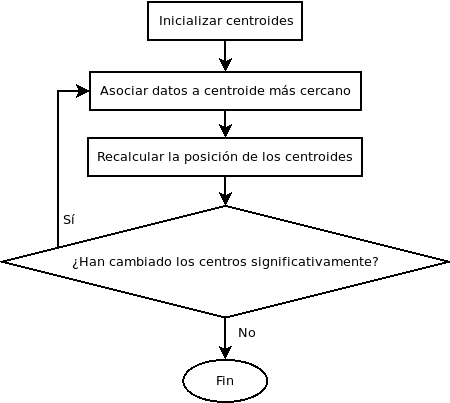
\includegraphics[width=0.7\textwidth]{agrupamiento-clasico.png}
				\label{clustering-algorithm}
				\caption{Proceso de agrupamiento clásico}
			\end{figure}
		
			Describamos ligeramente el proceso ilustrado arriba:
			
			\subsection{Inicialización de centroides}
			
				Consiste en colocar los centroides de forma generalmente aleatoria, dado que tomarán una posición más relevante a lo largo del proceso, conforme se vayan asignando datos a sus clases.\\
				
				La decisión más importante aquí es el número de centroides que se utilizan, aunque esta decisión goza de fácil solución si repetimos el algoritmo para distinto valor de este número, como podemos ver en la siguiente imagen:
				
				\begin{figure}[h]
					\centering
					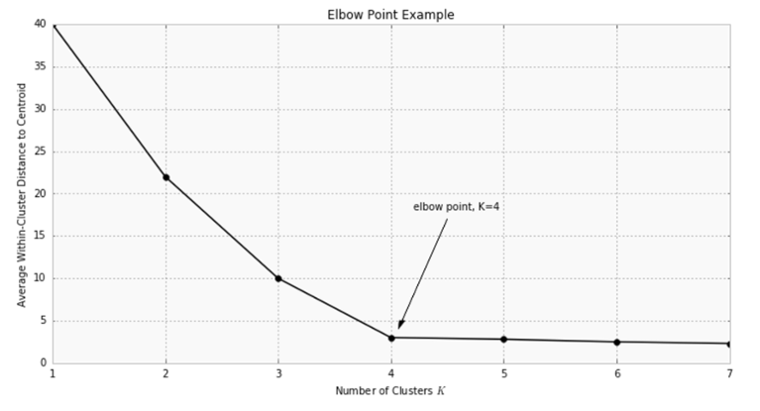
\includegraphics[width=0.9\textwidth]{k-means-oracle.png}
					\label{k-means-elbow-point}
					\caption{Inferencia del número idóneo de centroides a usar en un estudio de agrupamiento - \href{https://www.datascience.com/blog/k-means-clustering}{\textit{Oracle+DataScience}}}
				\end{figure}
				
				La opción más general reside en repetir el proceso del algoritmo aumentando ligeramente el número de centroides usados, hasta llegar al punto de inflexión donde aumentar este valor no produce una mejora demasiado notable, dado que conforme se incrementa el valor \textit{K}, así lo hace la capacidad computacional requerida para tratar el problema.
				
			\subsection{Clasificación de datos según centroide más cercano}
			
				Para seguir el modelo basado en centroide, cada uno de los datos presentes en el conjunto se asocia a la clase de la que es representativo el centroide más cercano o similar a dicho dato. Dependiendo del algoritmo, este criterio de asignación a categorías obviamente diferiría en cierto aspecto, pudiendo basarse esta decisión en alguna función de distancia de las comentadas previamente.
			
			\subsection{Reposicionamiento de los centroides}
			
				Dado que los centroides se conocen como los datos más representativos de un grupo, tras producirse cambios en los integrantes de esta categoría, la identidad o descripción de dicho centro probablemente se habrá visto alterada, por lo que deberán recalcularse y reflejarse en el modelo.\\
				
				Esto a su vez generará que en las próximas iteraciones los datos puedan cambiar a su vez de centroide más cercano, lo que conllevará una vez más otro reposicionamiento de los centros. Este hecho, como puede apreciarse, podría derivar en un proceso eterno sin convergencia, anulando la efectividad del algoritmo y requiriendo de alguna otra técnica de análisis.
			
			\subsection{Condición de parada}
			
				El criterio de finalización del algoritmo recae directamente sobre el resultado del apartado anterior, de forma que se considera que el proceso converge y termina cuando los centroides no alteran su posición tras la iteración completa, o bien la alteración es mínima. Como se viene comentando, esta convergencia final puede no encontrarse nunca, como se enumera en las limitaciones de este ejemplo de algoritmo.
				
		\section{Limitaciones}
		
			Lógicamente, estas aproximaciones basadas en agrupamiento clásico sufren de algunas limitaciones:
			
			\begin{itemize}
				\item Cada uno de los datos del conjunto solo pueden pertenecer a un \textit{cluster} (o lo que es lo mismo, ser asignados a una clase). Lógicamente no se contempla la posibilidad de que un elemento pueda compartir similitud gradual con diversas categorías, lo que aleja el estudio de los datos de la posible solución más favorable o descriptiva.
				
				\begin{figure}[h]
					\centering
					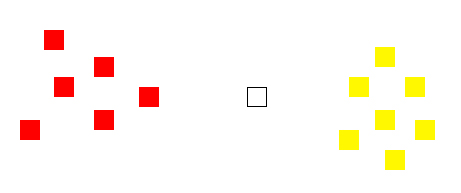
\includegraphics[width=0.5\textwidth]{Artboard1.jpg}
					\label{clustering2}
					\caption{Problema en la asignación de un dato en clustering clásico. ¿Qué categoría asignar al punto blanco?}
				\end{figure}
			
				\item Los mecanismos de exploración y clasificación de los datos no aseguran \textbf{convergencia}. El continuo cálculo de los centroides podría mantenerse eternamente efectuando las mismas operaciones repetitivas cuyo reposicionamiento de estos datos representativos alternase siempre de igual forma. Si existiese un mecanismo que permitiese relajar esta limitación, la inferencia extraída finalmente del estudio sería más descriptiva y ajustada a los datos reales.
			\end{itemize}
	
	\chapter{Agrupamiento difuso}
		Tal y como se acaba de ver, el agrupamiento clásico tiene una limitación bastante importante y es la de que un dato sólo puede pertenecer a un \textit{cluster}. Esto también tiene la consecuencia de que, dependiendo del algoritmo de agrupamiento que se vaya a emplear, no se puede garantizar la convergencia del mismo.\\
		
		A demás, si se usan redes neuronales para llevar a cabo la labor de agrupar los datos, es natural y lógico pensar que un sólo dato va a provocar la activación de más de una neurona. Es por ello que se tiene que cambiar el modelo clásico a uno más permisivo en el cual se solucionen dichos problemas.
			
		\section{Definición}
			Como se ha dejado entrever, el agrupamiento difuso permite que un dato pueda pertenecer a varios \textit{clusters} a la vez. Esto es posible debido a que al modelo clásico se le añade el concepto de \textit{función de pertenencia} que es propio de la lógica difusa.\\
			
			De hecho, en este modelo, un dato tiene $C$ grados de pertenencia, siendo $C$ el número de \textit{clusters} en los que se quiere agrupar los datos. La única limitación que tiene este modelo es que la sumatoria de los grados de pertenencia de un dato tiene que ser 1, es decir:
			
			$$\sum_{i=1}^c\mu_i(x_j) = 1, \forall j$$
			
			luego: $0 \leq \mu_i(x) \leq 1, \forall i=1,...,C$, es decir, el grado de pertenencia de cualquier dato en un \textit{cluster} tiene que estar en el intervalo cerrado [0,1].\\
			
			No obstante, la función objetivo que el agrupamiento clásico quiere minimizar no varía en su esencia:
			
			$$J_m(U,v) = \sum_{k=1}^n \sum_{i=1}^c (u_{ik})^m d^2_{ik}$$

			siendo:
			\begin{itemize}
				\item $d^2_{ik}$ la distancia entre los elementos y los centroides de los grupos calculada de igual manera que en el agrupamiento clásico ($d^2_{ik} = ||x_k-v_i||^2$, siendo $v$ el vector de controides).
				\item $(u_{ik})^m$ el grado de pertenencia asociado a cada distancia elevado a la m-ésima potencia. Cuando $m$ tiende a 1 ($m \rightarrow 1$) el modelo funcionaría cada ves más co mo un modelo clásico, mientras que si $m \rightarrow \infty$ el modelo no daría ningún resultado debido a que el grado de pertenencia de todos los elementos sería $1/C$.
			\end{itemize}
		
			Para el cálculo de $U$ previamente se necesitan tener calculados los centroides tal y como se hace en el método clásico. Una vez se tiene calculado el vector $v$, el cálculo de los componentes de $U$ se realizaría aplicando:
			
			$$u_{ik} = (\sum_{j=1}^c(\frac{d _{ik}}{d_{jk}})^{\frac{2}{m-1}})^{-1} ; 1 \leq x \leq n; 1\leq i \leq c $$
		
			Si se compara este modelo con el anterior se puede observar que sólo se añade el grado de pertenencia, como se ha dicho anteriormente, por lo que en el proceso del algoritmo se debería incluir el cálculo de dichos grados de pertenencia que se pueden poner en forma matricial con lo que el algoritmo quedaría esquematizado como se muestra en la figura \ref{agrupamiento_difuso}.
			
			\begin{figure}[h]
				\centering
				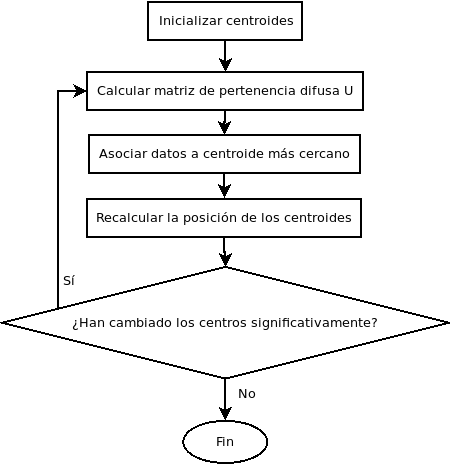
\includegraphics[width=0.7\textwidth]{agrupamiento-difuso.png}
				\label{agrupamiento_difuso}
				\caption{Proceso de agrupamiento clásico.}
			\end{figure}
		
			\subsection{Aplicación}
						
				El ejemplo anterior que no se ha podido resolver con el modelo clásico, se va a tratar de resolver con este nuevo enfoque. Como se vio en el ejemplo, el dato situado en medio de los dos grupos no se sabía a cual de ellos pertenecía.\\
				
				Ahora, tras meter grados de pertenencia se puede resolver de manera trivial como se muestra en la siguiente figura:
				
				\begin{figure}[h]
					\centering
					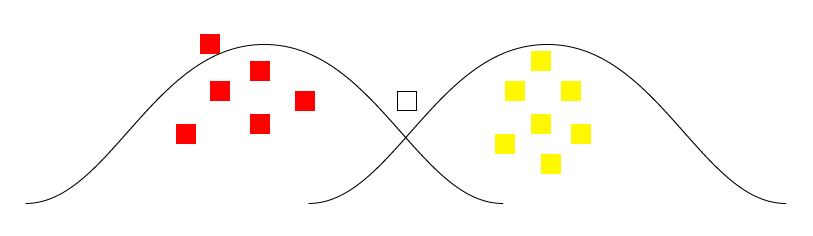
\includegraphics[width=0.5\textwidth]{clustering_difuso.jpg}
					\label{clustering_difuso}
					\caption{Ilustración de ejemplo de la función de pertenencia en Agrupamiento Difuso.}
				\end{figure}
			
				Como se puede observar gráficamente en la figura \ref{clustering_difuso}, cada \textit{cluster} forma una función de pertenencia centrada en el \textit{centroide} del mismo. Conforme se aleja del \textit{centroide} la función de pertenencia disminuye y se puede observar como el dato que se encuentra entre los dos grupos toma el mismo valor de pertenencia en los dos grupos.\\
				
				Este hecho da la información de que realmente ese dato se clasificaría diferente si se aumenta el números de \textit{clusters} a 3. Para entender esto se propone el siguiente ejemplo.\\
				
				Imaginemos que se quieren agrupar vehículos en dos clases: una clase \textit{turismo} y otra \textit{camión}. En el momento de clasificar una \textit{furgoneta}, sería imposible clasificarla en uno de estos dos grupos debido a que, en realidad, una \textit{furgoneta} es una mezcla entre un \textit{turismo} y un \textit{camión}, lo que sería otra clase distinta a estas.\\
				
				Dicho esto, el dato del ejemplo de la figura se puede comparar con la \textit{furgoneta} con lo que se le podría dar un color naranja, mezcla entre rojo y amarillo. Dicho color sería más rojo si el dato se acercase al grupo rojo o más amarillo en caso contrario.
				
				\begin{figure}[h]
					\centering
					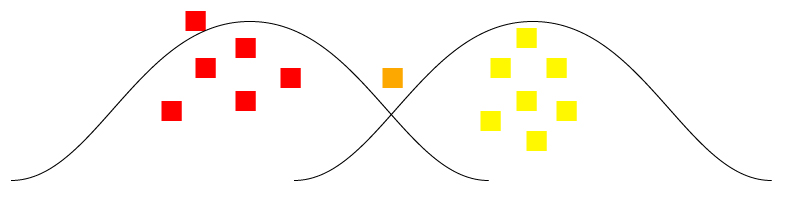
\includegraphics[width=0.5\textwidth]{clustering_difuso_solucion.jpg}
					\label{clustering_difuso_solucion}
					\caption{Ilustración de ejemplo resuelta tras usar Agrupamiento Difuso.}
				\end{figure}
		
		\section{Limitaciones}
		
			Aunque este modelo ha resuelto el problema de clasificar un dato que se encuentra entre dos o más grupos totalmente definidos, tiene deficiencias debido a la dureza de su restricción $\sum_{i=1}^c\mu_i(x_j) = 1, \forall j$.\\
			
			El caso más visible donde este modelo encuentra limitaciones se produce cuando en los datos hay los llamados \textit{outliers}. Estos son datos que por error de medición o porque realmente es un dato que se sale de la población son distantes al resto de datos, lo que genera mucha variabilidad en los mismos.\\
			
			Para ver de forma más clara esta limitación, se ha decidido realizar la siguiente ilustración que añade un nuevo dato \textit{outlier} a los datos que ya se habían clasificado previamente.
			
			\begin{figure}[h]
				\centering
				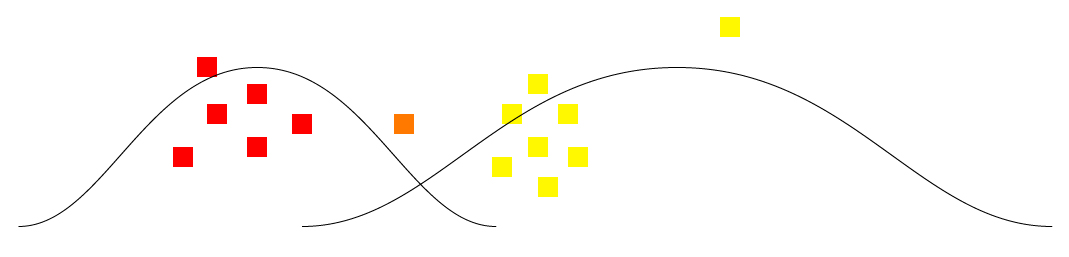
\includegraphics[width=0.5\textwidth]{problema-agrupamiento-difuso.jpg}
				\label{clustering_difuso_problema}
				\caption{Ilustración de ejemplo de la limitación del Agrupamiento Difuso.}
			\end{figure}
			
			Como se puede apreciar en la figura \ref{clustering_difuso_problema}, la función de pertenencia del conjunto de los puntos amarillos se tiene que extender de forma lógica para satisfacer la restricción de que la sumatoria de grados de pertenencia del punto más alejado tiene que ser 1. De esta manera, este punto, que a simple vista no pertenecería al grupo, entra a formar parte del núcleo o \textit{core} del conjunto. Esto implica que otros puntos ya no formarían parte del \textit{core} teniendo un menor grado de pertenencia en el grupo.\\
			
			El punto que anteriormente se había pintado naranja, ahora su tonalidad sería más rojiza debido al desplazamiento de la función de pertenencia del grupo amarillo. Este es un ejemplo con dos grupos pero, si hubiese más grupos el impacto de este \textit{outlier} sería más grande.
	
	\chapter{Agrupamiento difuso posibilístico}
	
		A pesar de que el agrupamiento difuso corrige ciertas limitaciones que tiene el agrupamiento clásico, este modelo no es del todo perfecto. Como se ha comprobado, los \textit{outliers} afectan muy negativamente al modelo de agrupamiento difuso al tener una restricción tan fuerte.\\
		
		Es por este motivo el nacimiento de un nuevo modelo para corregir las deficiencias del anterior en conjuntos de datos con ruido.
	
		\section{Definición}
		
		Al igual que el modelo de agrupamiento difuso, este permite que un dato pueda pertenecer a varios \textit{clusters} a la vez con cierto grado de pertenencia. La diferencia de este modelo con el anterior es que la sumatoria de los grados de pertenencia de un dato no tiene que ser uno.
		
		Esta condición se relaja de tener que ser estrictamente 1 a exigir solamente que al menos uno de los grados de pertenencia sea positivo, más concretamente estar comprendido en un intervalo [0,1], es decir:
		
		$$ 0 \leq \sum_{i=1}^c\mu_i(x_j) \leq 1, \forall j $$
		
		Con esta condición relajada, la función objetivo del agrupamiento difuso, $J_m(U,v) = \sum_{k=1}^n \sum_{i=1}^c (u_{ik})^m d^2_{ik}$, se resolvería trivialmente dando como resultado todo los valores de pertenencia a cero con lo que el modelo no sirve para nada. Para arreglar esto, a dicha función objetivo se le añade un nuevo término quedando:
		
		$$J_m(U,v,\eta) = \sum_{k=1}^n \sum_{i=1}^c (u_{ik})^m d^2_{ik} + \sum_{i=1}^c \eta _i \sum_{k=1}^n (1-i_{ik})^m$$
		
		Siendo el nuevo vector $\eta = (\eta_1,...,\eta_C)$ de valores positivos la distancia desde los centroides a la que el grado de pertenencia de un dato es 0.5. Este vector se calcula usando la siguiente fórmula:
		
		$$\eta_i = K \frac{\sum_{j=1}^n u_{ij}^m d_{ij}^2}{\sum_{j=1}^n u_{ij}^m}$$
		
		Donde $K$ es normalmente 1.
		
	\chapter{Aplicaciones reales}
	
		La parte teórica de una técnica no es más que un hecho meramente descriptivo si no se utiliza de forma real para resolver problemas existentes en la sociedad, por lo que para justificar este método de empleo de la lógica difusa se comentarán algunos casos de uso verdaderos donde este agrupamiento facilita la categorización de múltiples variantes de datos.\\
		
		\section{Agrupamiento difuso en el campo de la medicina}
		
			En el ámbito clínico, el número de patologías existentes no es fijo, dado que las bacterias y virus evolucionan a diario dando lugar a nuevas enfermedades que afectan a la sociedad de forma acuciante y a menudo inesperada. Es por esto que un análisis médico de síntomas podría no saber clasificarlos de forma unívoca a una enfermedad u otra, ya que puede darse el caso donde el paciente sufra una enfermedad que combina síntomas y efectos de diversas patologías.\\
			
			Para poner remedio a esto, en un entorno tecnológico e informatizado, mediante agrupamiento difuso se pueden estudiar dichos síntomas y asignarlos de forma gradual a las distintas enfermedades encontradas, como vemos en el caso de estudio de \textit{Fuzzy C-Means Clustering on Medical Diagnostic Systems} \cite{medicine}.\\
			
			Este artículo de investigación versa sobre métodos de agrupamiento no supervisado centrado en el desarrollo de un sistema de diagnóstico médico, utilizando la versión lógicamente difusa del algoritmo \textit{K-Means} (conocido como \textit{C-Means}) para evaluar a los pacientes y asignarles las diferentes enfermedades relacionadas con tiroides. Finalmente, se comparan estos resultados con los ofrecidos por un método tradicional basado en \textit{K-Means} para probar la efectividad de estas nuevas técnicas.
			
		\section{Lógica difusa aplicada al marketing e investigación de negocios}
		
			En una sociedad tan numerosa a la par que globalizada, las empresas que desean vender han de trabajar duro a diario para conseguir recomendaciones prolíficas que guíen a los potenciales clientes hasta sus productos. Sin embargo, con tan alto volumen de compañías como existe a diario, es difícil hacerse ver entre la niebla y llegar directamente al \textit{target} de gente que mejor se corresponde con lo que se pretende vender.\\
			
			Para esto se requiere de avanzadas técnicas de segmentación de mercados que doten de visibilidad a estas empresas, para las cuales es difícil siempre prever los gustos más característicos de la gente, que no son únicos y siempre se corresponden de forma gradual con sus intereses.\\
			
			Aquí encontramos otro interesante caso de estudio con la lógica difusa altamente implicada titulado \textit{Market definition and segmentation using fuzzy clustering methods} \cite{marketing}; donde se percibe a los diferentes potenciales clientes como un cúmulo de datos que los relaciona según su preferencia con las distintas marcas existentes en el mercado, aportando a los investigadores ciertas pistas sobre los intereses que mueven a las masas de compradores (y por tanto, al resto de gente que comparte gustos con ellos).\\
			
			Dicho estudio también combina técnicas clásicas y difusa de métodos de agrupamiento, esta vez para formar segmentos homogéneos de clientes y conjuntos de marcas competidoras para llegar a ellos de la forma más exitosa posible.
			
		\section{Técnicas de clustering difuso para recomendaciones en redes sociales}
		
			Las redes sociales componen una parte importante de la vida occidental hoy en día, siendo tanto una fuente de información para los usuarios finales como de ingresos para las empresas que orientan su negocio a través de esta \textit{relativamente} nueva forma de representación de Internet; que permite alcanzar altos niveles de audiencia mediante la viralización de contenidos multimedia o simplemente mensajes de texto, a mucho menor coste y con una velocidad de propagación mayor que con medios menos modernos como la televisión o los periódicos.\\
			
			Al igual que con la investigación de mercados, la presencia de publicidad en redes sociales ha de corresponderse con el mejor volumen de intereses presentes en los usuarios que las utilizan, por lo que conforman otro posible enfoque de la utilización de técnicas de agrupamiento difuso para crear visibilidad de un producto o fuente de información.\\
			
			Otra de estas aproximaciones la encontramos en una tesis titulada \textit{Fuzzy clustering in Social Networks - Fuzzy Student Recommender System} \cite{recommendation}, que una vez más utiliza estas técnicas comentadas para llegar a un foco de público basado en la información inferida a través de Internet y las redes sociales que lo integran.
			
\bibliographystyle{plain}
\bibliography{citas}

\end{document}          
